\documentclass[aspectratio=169]{beamer}

\usetheme{default}
\setbeamertemplate{navigation symbols}{}

\usepackage{graphicx}
\usepackage{booktabs}

\title{Kernel Composition Summary}
\author{}
\date{6 February 2026}

\begin{document}

\begin{frame}
  \titlepage
\end{frame}

\begin{frame}{Overview}
  \begin{itemize}
    \item Summarizes kernel composition experiments.
    \item Compares composition runs against prior MMR/ABESS baselines.
    \item Highlights best-performing configuration and key visuals.
  \end{itemize}
  \vspace{0.5em}
  \small This deck focuses on how composition size and per-family bank size affect test AUC/ACC.
\end{frame}

\begin{frame}{Composition Results}
  \begin{center}
    \begin{tabular}{lccc}
      \toprule
      Run & Test AUC & Test ACC & Comp. pool \\
      \midrule
      A & 0.8662 & 0.7968 & 25 \\
      B & 0.8666 & 0.7920 & 125 \\
      C & 0.8869 & 0.8107 & 625 \\
      D & 0.8933 & 0.8150 & 1250 \\
      \bottomrule
    \end{tabular}
  \end{center}
  \vspace{0.5em}
  \small Larger composition pools improve composite test AUC/ACC; D is strongest.
\end{frame}

\begin{frame}{Composite Kernel Visualization}
  \begin{center}
    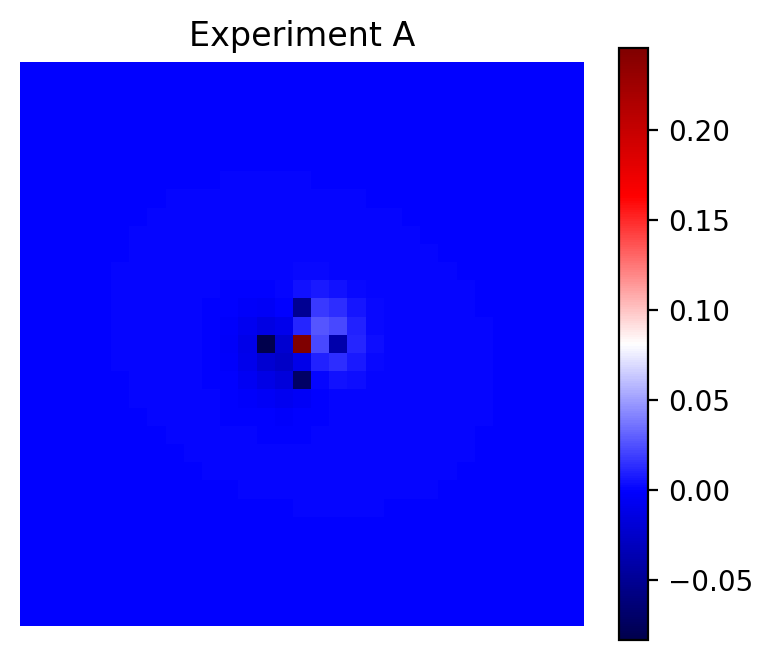
\includegraphics[width=0.48\linewidth]{../../results/exp_022_mmr_nperFamily10_nComposition25/composite_kernel.png}
    \hfill
    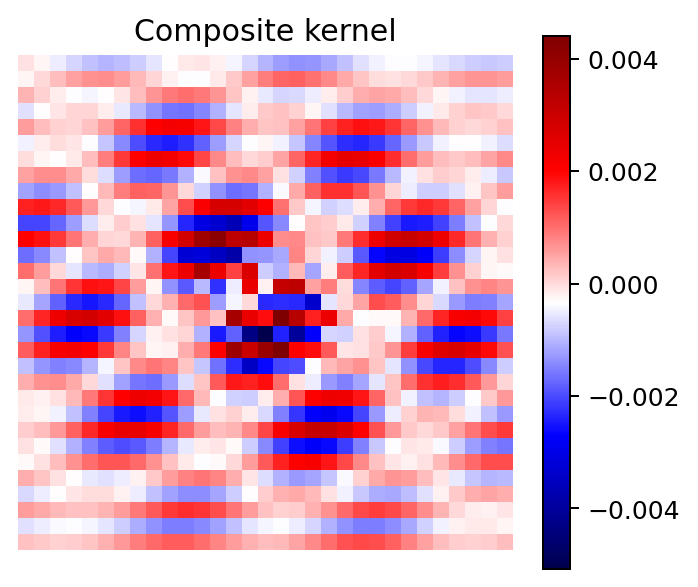
\includegraphics[width=0.48\linewidth]{../../results/exp_022_mmr_nperFamily500_nComposition1250/composite_kernel.png}
  \end{center}
  \vspace{0.5em}
  \small Red/blue indicate positive/negative response regions; stronger contrast suggests a more selective filter.
\end{frame}

\begin{frame}{Heatmap Example (Best Composition)}
  \begin{center}
    % results/exp_022_mmr_nperFamily500_nComposition1250/heatmaps_side_by_side.png
    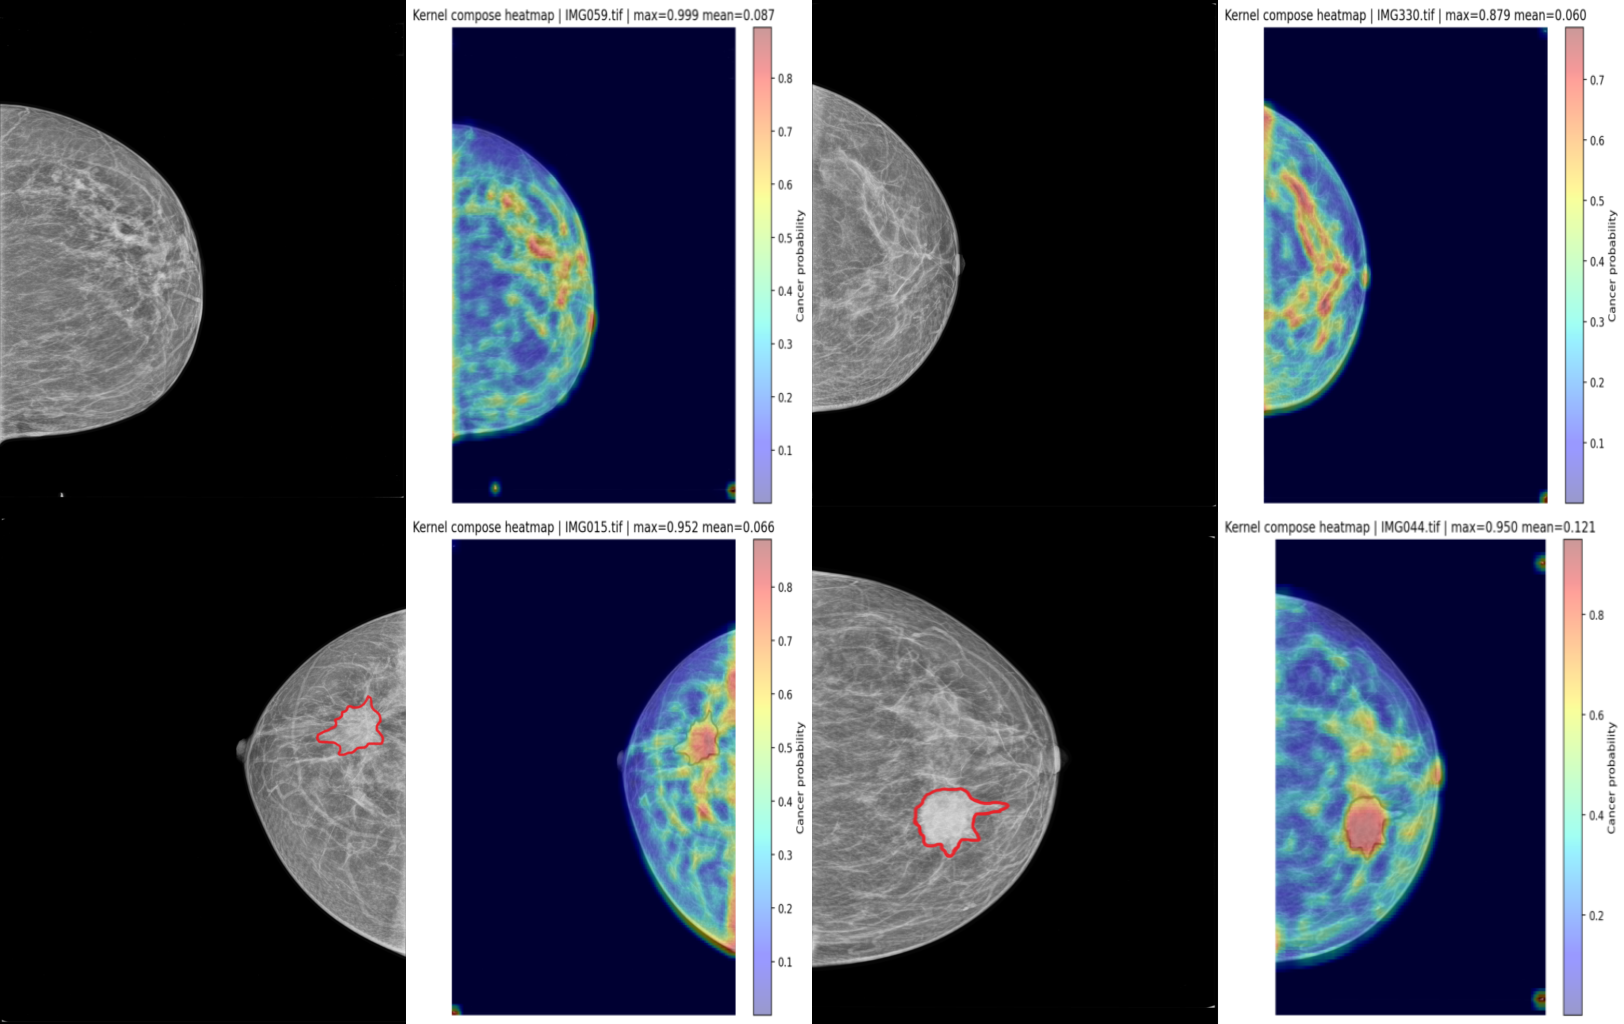
\includegraphics[width=0.95\linewidth]{../../results/exp_022_mmr_nperFamily500_nComposition1250/heatmaps_side_by_side.png}
  \end{center}
  \vspace{0.5em}
  \small The composed kernel highlights malignant regions with higher probability while keeping healthy regions cooler.
\end{frame}

\section*{How parameter changes affect quality}
\begin{frame}{How parameter changes affect quality}
  \begin{itemize}
    \item Increasing composition size (25 $\rightarrow$ 125) improves both test AUC and test accuracy.
    \item Increasing per-family kernel count (10 $\rightarrow$ 50) yields a stronger composite filter and better generalization.
    \item Smaller banks keep accuracy competitive but usually reduce AUC.
    \item Best quality comes from a larger kernel bank and a larger composition size.
  \end{itemize}
\end{frame}

\begin{frame}{Composition vs non-composition accuracy}
  \begin{center}
    \begin{tabular}{lcc}
      \toprule
      Run & Test ACC (regular) & Test ACC (composite) \\
      \midrule
      A & 0.8487 & 0.7968 \\
      B & 0.8503 & 0.7920 \\
      C & 0.8492 & 0.8107 \\
      D & 0.8733 & 0.8150 \\
      \bottomrule
    \end{tabular}
  \end{center}
  \vspace{0.5em}
  \small Regular models score higher, while composites provide a stable, interpretable baseline.
\end{frame}

\begin{frame}{Conclusion}
  \begin{itemize}
    \item Best overall: run D (500 per-family, 1250 composition).
    \item Highest composite test AUC (0.8933) and composite test ACC (0.8150).
    \item It also delivers the best regular-model test accuracy (0.8733).
  \end{itemize}
\end{frame}

\begin{frame}{Next Steps}
  \begin{itemize}
    \item Run more experiments with different parameter settings to improve accuracy.
    \item Test on a new dataset to confirm generalization.
    \item Study a learned kernel-generating model to avoid random kernel sampling.
  \end{itemize}
\end{frame}

\begin{frame}{Recommendation}
  \begin{itemize}
    \item Prefer a single composite kernel over a large uncombined kernel bank.
    \item It performs better in prior runs while being simpler and faster to deploy.
    \item Keep the large multi-kernel model only as a reference baseline.
  \end{itemize}
\end{frame}

\end{document}
